\documentclass{standalone}
\usepackage{tikz}
\usepackage{amsmath}

\begin{document}
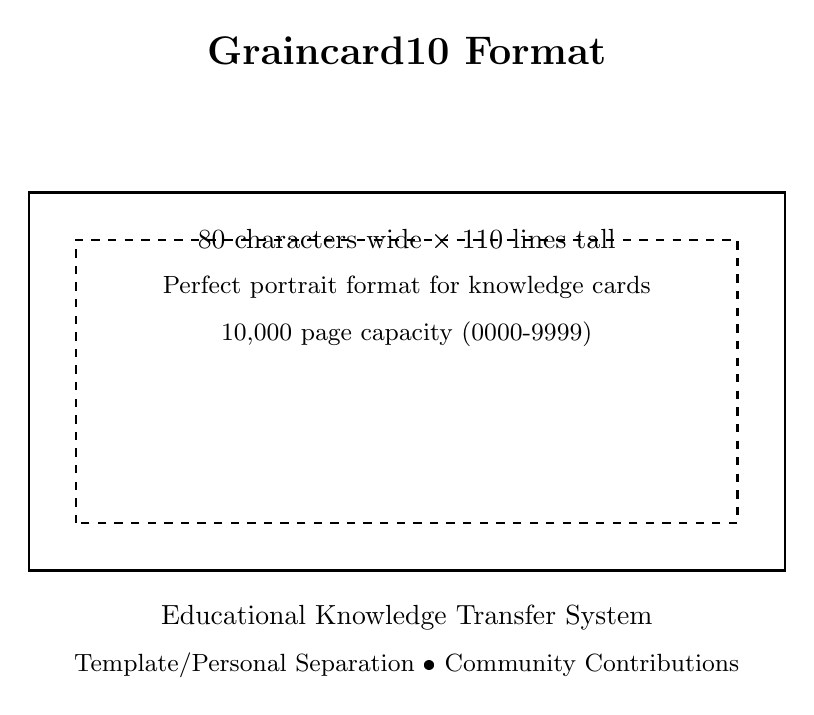
\begin{tikzpicture}[scale=1.2]
    % Title
    \node[font=\Large\bfseries] at (0, 3.5) {Graincard10 Format};
    
    % Card outline
    \draw[thick] (-4, -2) rectangle (4, 2);
    
    % Card content
    \node[font=\normalsize] at (0, 1.5) {80 characters wide × 110 lines tall};
    \node[font=\small] at (0, 1) {Perfect portrait format for knowledge cards};
    \node[font=\small] at (0, 0.5) {10,000 page capacity (0000-9999)};
    
    % Decorative border
    \draw[thick, dashed] (-3.5, -1.5) rectangle (3.5, 1.5);
    
    % Bottom text
    \node[font=\normalsize] at (0, -2.5) {Educational Knowledge Transfer System};
    \node[font=\small] at (0, -3) {Template/Personal Separation • Community Contributions};
\end{tikzpicture}
\end{document}
